各々の入射方向に対して得られた波形データから、群速度$<c_g>,\bar c_g$と
相互相関速度$<c_{cor}>, \bar c_{cor}$を計算した結果を図\ref{fig:fig12}に示す。
この図では、横軸は入射方向を縦軸に音速値(km/s)を示している。
音速値は、概ね2.7(km/sec)から3.15(km/sec)の範囲にあり、主として表面波からなる
波動が観測されていることが分かる。
この中で最も方向による変化が大きいのは平均群速度$<c_g>$であった。
$\theta=150$度と330度の方向で極大、$\theta=30,240$度の方向で極小
となっており、明らかな音響異方性を示している。
一方、平均波形$<a>(t)$から求めた群速度$\bar c_g$の方向による変動幅は
0.1(km/sec)と小さく、波形の平均化により速度の異方性が弱められることを示している。
また、相互相関速度$,<c_{cor}>$と$\bar{c}_{cor}$の挙動は、$\bar c_g$のそれと
欲似ている。相互相関関数の計算では、参照波形として用いた入射波波形と
よく似た波形の到達時間を検出する。そのため、最もよく位相が揃った波動が到達する
時刻が得られるものの、観測点毎の速度の変動を反映しにくいと考えられる。
以上のことから、音響異方性の評価には、局所的な群速度の平均$<c_g>$を見ることが
よいと考えられる。
%--------------------
\begin{figure}[h]
	\begin{center}
	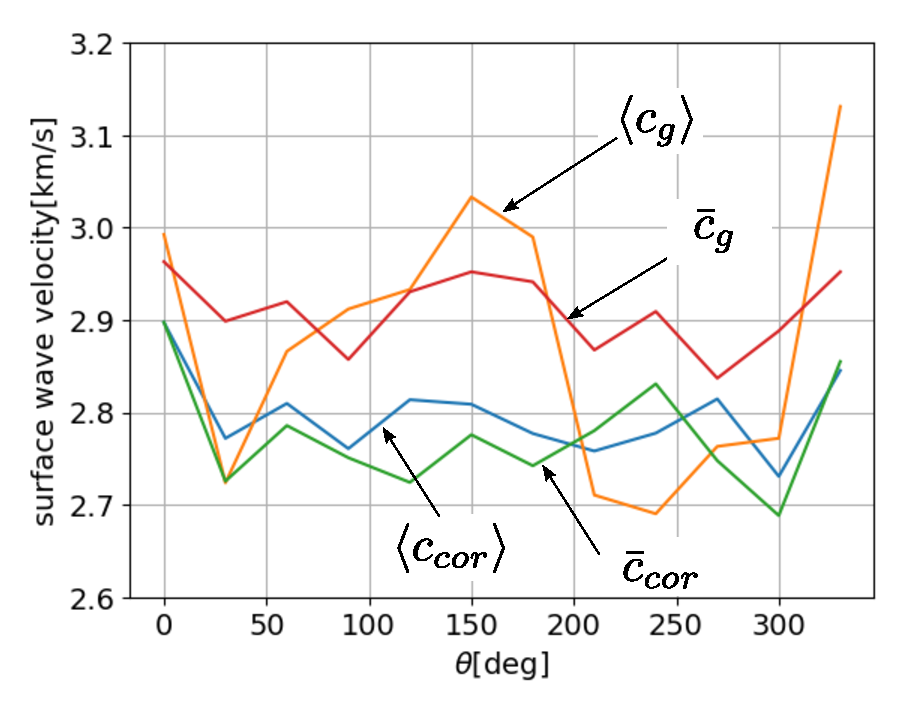
\includegraphics[width=0.8\linewidth]{Figs/fig12.eps} 
	\end{center}
	\caption{
		入射方向による群速度と相互相関速度の変化.
	} 
	\label{fig:fig12}
\end{figure}
%--------------------

ここで、入射方向毎に得られた平均波形$<a>(t)$を一覧すると、
図\ref{fig:fig11_1}のようになっている。
これらの波形の振幅はLDV出力の電圧値(mV)だが、大小関係は波形相互に
比較が可能である。この結果に示されるように、平均波形の最大振幅は
明らかに方向によって変化している。そこで、
平均波形の最大振幅max$\left\{ \left< a \right>\right\}$と,
最大振幅の平均$\left< {\rm max}\left\{ a \right\} \right>$
の、入射方向による変化を調べると、図\ref{fig:fig14}のようになる。
この結果を図\ref{fig:fig12}と比べると、最大振幅の平均
$\left<{\rm max}\left\{a\right\}\right>$
は、$\left<c_g\right>$を上下に反転させたような形で、
強い異方性を示していることが分かる。
すなわち、群速度の速い方向で振幅は小さく、遅い方向では振幅が大きく
なっていることが分かる。これは、岩石供試体の見かけの剛性、30度と240度の
方向で小さく、150度と0度方向で大きくなっていると考えると整合的である。
なお、平均波形の最大振幅max$\left\{<a>\right\}$は
最大振幅の平均よりも変動が若干小さい。これは、
波動の到達時間の変動を考慮せずに最大値の平均をとる方が、
音響異方性をより直接的に反映した結果が得られることを意味している。
%--------------------
\begin{figure}[h]
	\begin{center}
	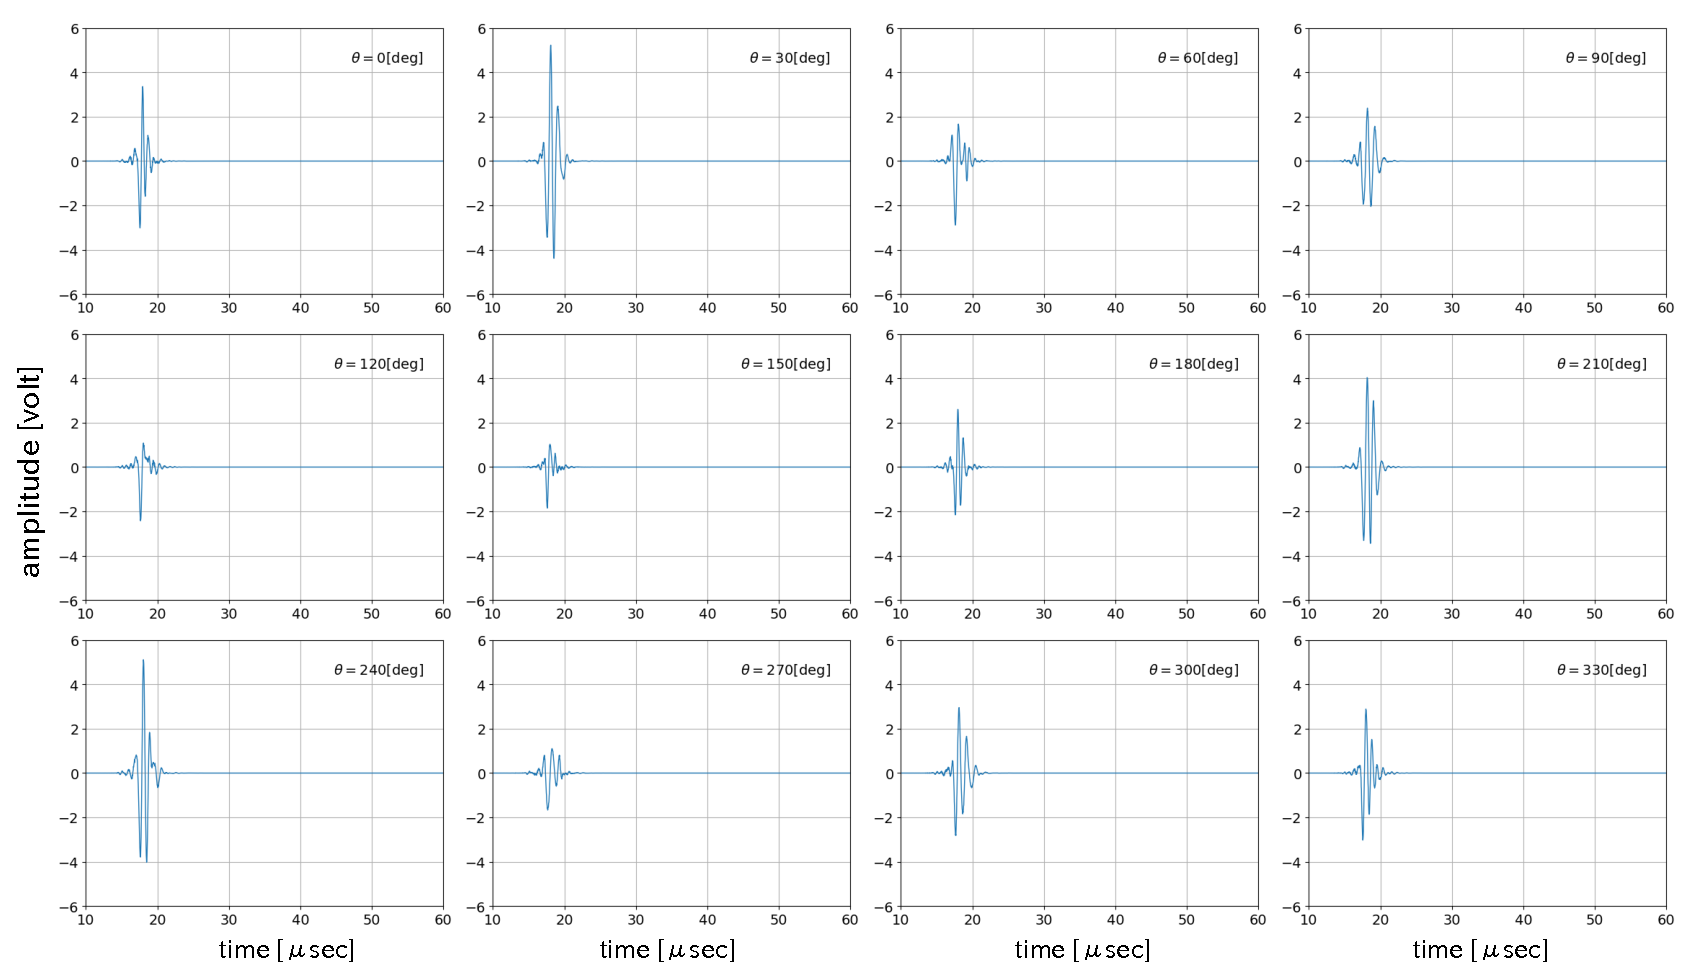
\includegraphics[width=1.0\linewidth]{Figs/fig11_1.eps} 
	\end{center}
	\caption{
		入射方向毎に得られた平均波形の時刻歴.
	} 
	\label{fig:fig11_1}
\end{figure}
%--------------------
\begin{figure}[h]
	\begin{center}
	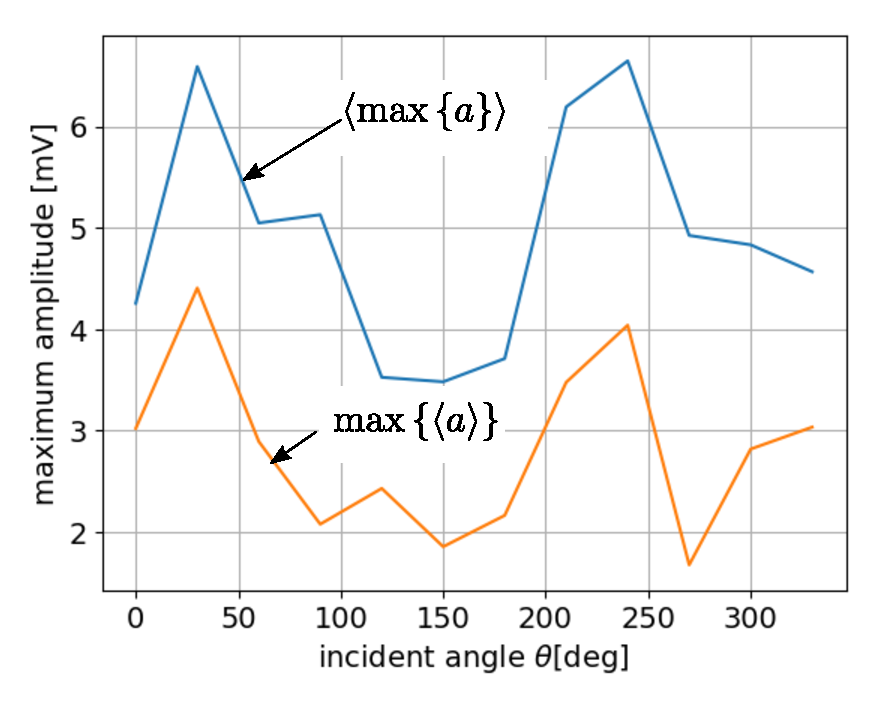
\includegraphics[width=0.8\linewidth]{Figs/fig14.eps} 
	\end{center}
	\caption{
		入射方向による最大振幅値の変化.
	} 
	\label{fig:fig14}
\end{figure}
最後に、平均波形の周波数スペクトル
\begin{equation}
	\left< A \right> (\omega) = \int \left<a\right>(t)e^{-i\omega t}dt
	\label{eqn:ave_A}
\end{equation}
を入射方向毎に計算した結果を示すと、図\ref{fig:fig11_2}のようになる。
これらの結果を見ると、周波数帯域はいずれの方向でも3MHz程度までで大きな違いは無いが、
ピーク周波数にはばらつきがあることが分かる。そこで、平均波形の
ピーク周波数argmax$\left< A \right>$と,個々の観測波形のピーク周波数の平均
$\left< {\rm argmax }\left\{ A \right\}\right>$を求め、角度との関係を見ると、
図\ref{fig:fig13}のようになる。この図より、
ピーク周波数の平均$\left< {\rm argmax }\left\{ A \right\}\right>$は
$\left< c_g\right>$と似た傾向を示している。具体的には、
群速度平均が大きな方向では、ピーク周波数平均が高く、
群速度平均が小さな方向では、ピーク周波数平均は低くなることが分かる。
これは、見かけの剛性が高い方が、高周波の波を伝えやすく、剛性が低い方が
伝えにくいことを示す。ここで、見かけの剛性と周波数が相関することは、
剛性の変化がマイクロクラックに起因したものであることを示唆している。
なぜならば、均質材の場合、剛性の大小は振幅や音速には影響するが、
周波数応答には関与しないためである。剛性の周波数依存性は界面の接触や滑りに
関係している可能性が高く、この結果は弾性波を使ったき裂評価において有用な
情報であると考えられる。
なお、ピーク周波数の平均が、平均波形のピーク周波数よりも変動が小さい理由は
平均最大振幅と平均波形の最大振幅の大小に関する理由と同様である。
%--------------------
\begin{figure}[h]
	\begin{center}
	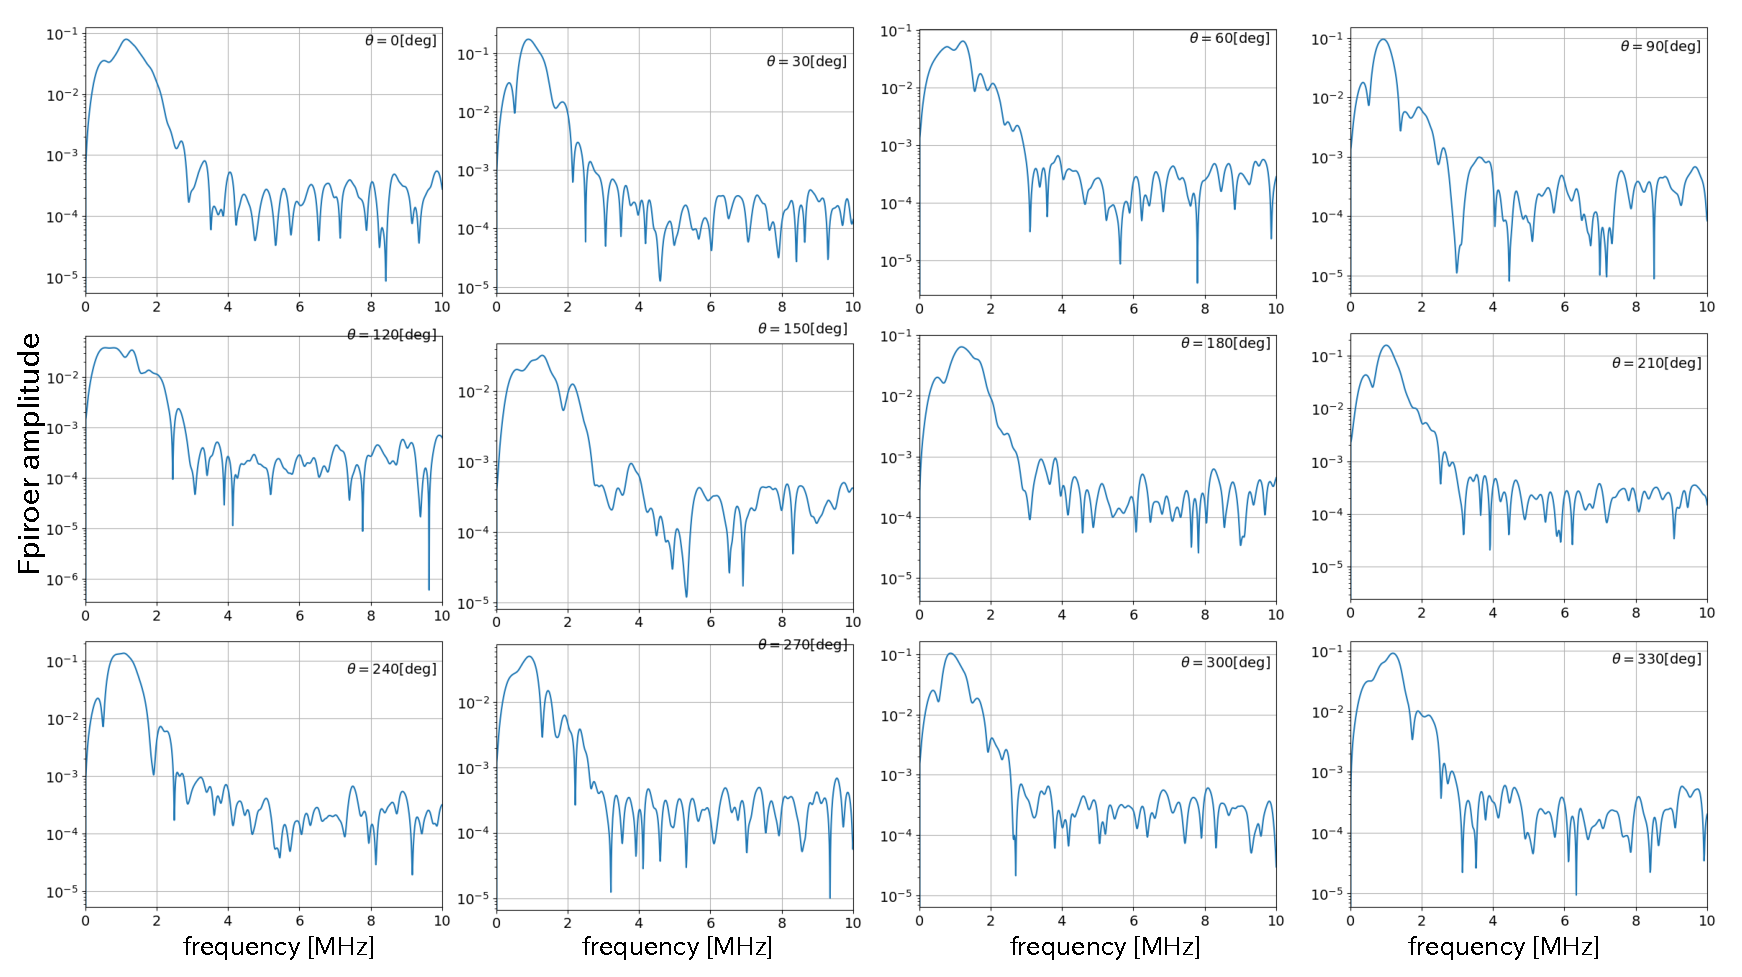
\includegraphics[width=1.0\linewidth]{Figs/fig11_2.eps} 
	\end{center}
	\caption{
		入射方向毎に得られた平均波形の周波数スペクトル.
	} 
	\label{fig:fig11_2}
\end{figure}
\begin{figure}[h]
	\begin{center}
	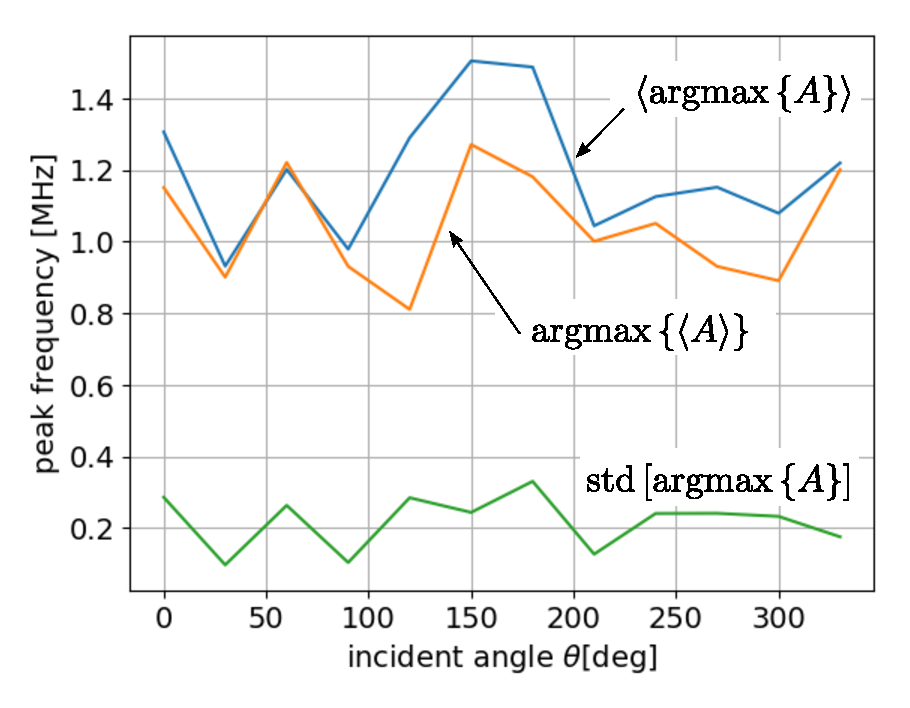
\includegraphics[width=0.8\linewidth]{Figs/fig13.eps} 
	\end{center}
	\caption{
		入射方向によるピーク周波の変化.
	} 
	\label{fig:fig13}
\end{figure}
%--------------------

